\documentclass[12pt,compress,aspectratio=169]{beamer}

\usetheme{metropolis}
\setbeamersize{text margin left=.5cm,text margin right=.5cm}

\usefonttheme{professionalfonts}
\usepackage{amsmath}
\usepackage{graphicx}
\usepackage{tikz}
\usepackage{mathpazo}
\usepackage{xcolor,colortbl}
%\usepackage{hyperref}
\usepackage{siunitx}
\usepackage{bm}

\setsansfont{Roboto Light}
\setmonofont{Ubuntu Mono}
\setlength{\parskip}{0pt}
\renewcommand{\baselinestretch}{1}

\sisetup{
  detect-all=true,
  %number-math-rm=\mathnormal,
  per-mode=symbol
}


\title{Topic 2: Dynamics}
\subtitle{Advanced Placement Physics 1}
\author[TML]{Dr.\ Timothy Leung}
\institute{Olympiads School}
\date{\today}

\newcommand{\pic}[2]{\includegraphics[width=#1\textwidth]{#2}}
\newcommand{\mb}[1]{\ensuremath\mathbf{#1}}
\newcommand{\eq}[2]{\vspace{#1}{\Large\begin{displaymath}#2\end{displaymath}}}

\begin{document}

\begin{frame}
  \maketitle
\end{frame}

\begin{frame}{Dynamics}
  While we use \textbf{kinematics} to describe the motion of any object
  mathematically, we use \textbf{dynamics} to describe \emph{what} causes
  motion (or more precisely, \emph{what causes motion to change?})
  \begin{itemize}
  \item Newton's three laws of motion
  \end{itemize}
\end{frame}



\section{Laws of Motion}

\begin{frame}{First Law of Motion}
  \textbf{Every body persists in its state of being at rest or moving uniformly
    straight forward, except insofar as it is compelled to change its state by
    force impress'd.}\footnote{Lex I: Corpus omne perseverare in statu suo
    quiescendi vel movendi uniformiter in directum, nisi quatenus a viribus
    impressis cogitur statum illum mutare.}
  
  \begin{itemize}
  \item ``Moving uniformly'' means \emph{uniform motion} with constant velocity
    \begin{itemize}
    \item An object ``at rest'' is also in uniform motion with $\mb{v}=\mb{0}$
    \end{itemize}
  \item As long as an object moves in uniform motion, it must be that
    $\mb{F}_\mathrm{net}=\mb{0}$
  \item Common examples:
    \begin{itemize}
    \item A hockey puck sliding on very smooth ice has gravity and normal
      force, but the net force is zero
    \item A car traveling on a highway at \SI{100}{\kilo\metre\per\hour}
      has many forces acting on it, but the net force is zero 
    \end{itemize}
  \end{itemize}
  \vspace{.2in}
\end{frame}


\begin{frame}{Second Law of Motion}
  \textbf{The alteration of motion is ever proportional to the motive force
    impress'd; and is made in the direction of the right line in which that
    force is impress'd.}\footnote{Lex II: Mutationem motus proportionalem esse
    vi motrici impressae, et fieri secundum lineam rectam qua vis illa
    imprimitur.}

  \vspace{.2in}The \emph{alteration of motion} means \emph{acceleration}. The
  first two laws of motion can be summarized in the equation:

  \eq{-.2in}{
    \boxed{\mb{F}_{\textrm{net}}=\Sigma\mb{F}=m\mb{a}}
  }
%  \begin{center}
%    \begin{tabular}{l|c|c}
%      \rowcolor{pink}
%      \textbf{Quantity} & \textbf{Symbol} & \textbf{SI Unit} \\ \hline
%      Net unbalanced force (sum of all forces)
%      & $\mb{F}_{\textrm{net}}$ & \si{\newton}\\
%      Mass         & $m$       & \si{\kilo\gram} \\
%      Acceleration & $\mb{a}$  & \si{m/s^2}
%    \end{tabular}
%  \end{center}

  \textcolor{red!80!black}{This equation is a ``special case'' that assumes a
    constant mass.}
\end{frame}


\begin{frame}{Third Law of Motion}
  \textbf{To every action there is always opposed an equal reaction: the
    mutual actions of two bodies upon each other are always equal, and directed
    to contrary parts.}\footnote{Lex III: Actioni contrariam semper et aequalem
    esse reactionem: sive corporum duorum actiones in se mutuo semper esse
    aequales et in partes contrarias dirigi.}
 
  %\vspace{.1in}For every action force on an object (B) due to another object
  %(A), there is a reaction force which is equal in magnitude but opposite in
  %direction, on object (A), due to object (B):

  \eq{-.2in}{
    \boxed{\mb{F}_{\text{AB}} = -\mb{F}_{\text{BA}}}
  }
  \begin{itemize}
  \item ``Contrary parts'' means the action and reaction forces act on
    different objects
  \item Third law is the natural consequence of the first and second law.
    Action/reaction forces are \emph{internal} forces.
  \end{itemize}
  \vspace{.2in}
\end{frame}


%\begin{frame}
%  \frametitle{Example Problem}
%  \framesubtitle{A Blast From the Past}
%  This problem can get you started to remember how to do these problems, but it
%  is a bit too easy for AP Physics.
%  
%  \vspace{.2in}\textbf{Example 1:} In old-style television picture tubes and
%  computer monitors (cathode ray tubes), light is produced when fast-moving
%  electrons collide with phosphor molecules on the surface of the screen. The
%  electrons (mass $m=\SI{9.1e-31}{kg}$) are accelerated from rest in the
%  electron ``gun'' at the back of the vacuum tube. Find the velocity of an
%  electron when it exits the gun after experiencing an electric force of
%  \SI{5.8e-15}{N} over a distance of \SI{3.5}{mm}.
%\end{frame}



\begin{frame}{Forces}

  A \textbf{force} is the interaction between the objects.
  \begin{itemize}
  \item When there is interaction, then forces are created
  \item A ``push'' or a ``pull''
%    \item Gravity: interaction between to objects with mass
%    \item Electric force: interaction between two charged object
%    \item Nuclear force: interaction between protons, electrons and neutrons
  \end{itemize}

  There are two broad categories of forces:
  \begin{itemize}
  \item\textbf{Contact forces} act between two objects that are in contact
    with one another
  \item\textbf{Non-contact forces} act between two objects without them
    touching each other. They are also called ``action-at-a-distance'' force
  \end{itemize}
\end{frame}



\begin{frame}{Center of Mass}
  \vspace{.2in}
  \begin{columns}
    \column{.7\textwidth}
    Newton considered all forces acting at a single point of an object called
    the center of mass (``CM'')
    \begin{itemize}
    \item The center of mass is also called the center of gravity (``CG''), if
      the entire object is inside a uniform gravitational field
    \item If the density of an object is constant, then the CM/CG is also the
      geometric center (centroid) of the object
    \end{itemize}

    \column{.3\textwidth}
    \pic{1}{graphics/cofm.png}
  \end{columns}
\end{frame}

\begin{frame}{Static \& Dynamic Equilibrium}
  If the net force on an object is zero ($\Sigma\mb{F}=\mb{0}$) then the
  object is in a \emph{state of equilibrium}
  \begin{itemize}
  \item Dynamic equilibrium: the object is moving relative to us
  \item Static equilibrium: the object is not moving relative to us
  \end{itemize}
\end{frame}


\section{Common Forces}

\begin{frame}{Common Forces}
  Common everyday forces that we encounter in Physics 12 include:
  \begin{itemize}
  \item Weight (gravitational force) $\mb{w}$ (or $\mb{F}_G$)
  \item Normal force $\mb{N}$
  \item Friction (static $\mb{f}_s$ and kinetic $\mb{f}_k$)
  \item Tension $\mb{T}$
  \item Applied force $\mb{F}_a$
  \item Spring force $\mb{F}_e$
  \item Drag $\mb{D}$ (fluid resistance, then again in fluid mechanics)
  \item Buoyant force $\mb{B}$ (discussed in fluid mechanics)
  \item Electrostatic force $\mb{F}_E$ (discussed in E \& M exam)
  \item Magnetic force $\mb{F}_M$ (discussed E \& M exam)
  \end{itemize}
\end{frame}



\begin{frame}{Gravity}
  Gravity is the force of attraction between all objects with mass
    
  \eq{-.2in}{
    \boxed{\mb{w}=m\mb{g}}
  }
  \begin{itemize}
  \item\vspace{-.15in}Near surface of Earth, use $g=\SI{9.81}{m/s^2}$ (or
    $g=\SI{10}{m/s^2}$ for your AP exam)
  \item You may be asked to find the value of $g$ on some ``unknown planet''.
  \item $\mb{w}$ always points \emph{down} (the direction of $\mb{w}$ is how
    down is defined)
%  \item Newton's law of universal gravity:
%
%    \eq{-.3in}{
%      \boxed{W=F_G=\frac{Gm_1m_2}{r^2}}\;\;
%      \text{\normalsize where}\;\;
%      G=\SI{6.67e-11}{N.m^2/kg^2}
%    }
  \end{itemize}    
\end{frame}



\begin{frame}{Normal Force}
  \begin{columns}
    \column{.22\textwidth}
    \begin{center}
      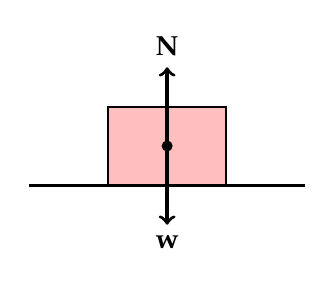
\begin{tikzpicture}{scale=1.5}
        \draw [very thick] (-1,0)--(2.5,0);
        \draw [fill=pink,thick] (0,0) rectangle (1.5,1);
        \fill (.75,.5) circle(2pt);
        \draw [->,very thick] (.75,.5)--(.75,-.5)
        node[pos=1,below]{$\mb{w}$};
        \draw [->,very thick] (.75,.5)--(.75,1.5)
        node[pos=1,above]{$\mb{N}$};
      \end{tikzpicture}
    \end{center}
    \begin{displaymath}
      \mb{w}=m\mb{g}=-\mb{N}
    \end{displaymath}
    
    \column{.78\textwidth}
    \begin{itemize}
    \item A force a surface exerts on another object that it is in contact with
    \item Always \emph{perpendicular} to the contact surface
    \item\textbf{Special case:} When an object is on a horizontal surface
      with no additional applied force, the magnitude of the normal force is
      equal to the magnitude of the weight of the object, i.e.\ $N=w$
    \end{itemize}
  \end{columns}
\end{frame}



\begin{frame}{Normal Force on a Slope}
  For this case, we label the $x$-axis to be along the slope, and $y$-axis to
  be perpendicular to the slope.
  \begin{columns}
    \column{.35\textwidth}
    \begin{center}
      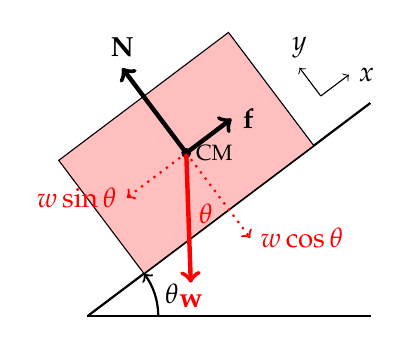
\begin{tikzpicture}[scale=.9]
        \draw[thick] (-1,0)--(3,0);
        \draw[thick,->](0,0) arc(0:37:1) node[midway,right] {$\theta$};
        \begin{scope}[rotate around={37:(-1,0)}]
          \draw[->](3.5,.5)--(4,.5) node[pos=1,right]{$x$};
          \draw[->](3.5,.5)--(3.5,1) node[pos=1,above]{$y$};
          \draw[thick] (-1,0)--(4,0);
          \draw[fill=pink] (0,0) rectangle (3,2);
          \fill(1.5,1) circle (2pt) node[right]{\footnotesize CM};
          \draw [->,thick,dotted,red] (1.5,1)--(1.5,-.5)
          node[pos=1,right]{$w\cos\theta$};
          \draw [->,thick,dotted,red] (1.5,1)--(.45,1)
          node[pos=1,left]{$w\sin\theta$};
          \draw [->,ultra thick,red] (1.5,1)--(.45,-.5)
          node[pos=1,below]{$\mb{w}$}
          node[pos=.3,below right]{$\theta$};
        \draw [->,ultra thick] (1.5,1)--(1.5,2.5) node[pos=1,above]{$\mb{N}$};
        \draw [->,ultra thick] (1.5,1)--(2.3,1) node[pos=1,right]{$\mb{f}$};
        \end{scope}
      \end{tikzpicture}
    \end{center}
    
    \column{.65\textwidth}
    \begin{itemize}
    \item If on a slope: $N=w\cos\theta$
      \begin{itemize}
      \item $N$ decreases as ramp angle $\theta$ increases
      \end{itemize}
    \item $w$ has a component along the ramp $w\sin\theta$ that wants to slide
      the block down.
    \item Friction force $f$ opposes the motion
      \begin{itemize}
      \item Be careful: if the block is moving \emph{up} the ramp with an
        applied force, then $f$ will point \emph{down} the ramp
      \end{itemize}
    \end{itemize}
  \end{columns}
\end{frame}



\begin{frame}{Friction}
  \textbf{Friction} is a force that opposes the sliding of two surface against
  one another
  \begin{itemize}
  \item Always act in a direction that opposes motion or attempted motion
  \item Depends on:
    \begin{itemize}
    \item The force the two surfaces are pressed against each other
    \item The smoothness of the surfaces, which itself depends on
    \item The material(s) the surfaces are made of
    \item The use of lubricants
    \end{itemize}
  \end{itemize}
  \begin{center}
    \pic{.6}{graphics/friction.png}
  \end{center}
\end{frame}



\begin{frame}{Static Friction}
  \textbf{Static friction} between the two surfaces is when there is no
  relative motion between them
  \begin{itemize}
  \item Increases with increasing applied force
  \item Maximum when the object is just about to move
  \end{itemize}

  \eq{-.35in}{
    \boxed{f_s\leq\mu_sN}
  }
  \begin{center}
    \begin{tabular}{l|c|c}
      \rowcolor{pink}
      \textbf{Quantity} & \textbf{Symbol} & \textbf{SI Unit} \\ \hline
      Magnitude of maximum static friction & $f_s$ & \si{\newton} \\
      Static friction coefficient  & $\mu_s$ & no units \\
      Magnitude of normal force    & $N$ & \si{\newton}
    \end{tabular}
  \end{center}
\end{frame}



\begin{frame}{Kinetic Friction}
  \textbf{Kinetic friction} between two surfaces is when they are moving
  relative to each other. $f_k$ is constant along the path of movement as long
  as $\mb{N}$ stays constant

  \eq{-.3in}{
    \boxed{f_k = \mu_kN}
  }
  \begin{center}
    \begin{tabular}{l|c|c}
      \rowcolor{pink}
      \textbf{Quantity} & \textbf{Symbol} & \textbf{SI Unit} \\ \hline
      Magnitude of kinetic friction & $f_k$ & \si{\newton} \\
      Kinetic friction coefficient  & $\mu_k$ & no units \\
      Magnitude of normal force     & $N$ & \si{\newton}
    \end{tabular}
  \end{center}
\end{frame}



\begin{frame}{Static and Kinetic Coefficients of Friction}    
  Kinetic friction coefficient is always lower than the static coefficient,
  otherwise nothing will ever move:
    
  \eq{-.45in}{
    \mu_k\leq\mu_s
  }

  \vspace{-.2in}Consider a simple case of a box being pulled along a level floor. The
  free-body diagram is simple (left). How do the magnitudes of the applied
  force $F_a$ and friction $f$ compare?

  \vspace{-.2in}
  \begin{columns}
    \column{.4\textwidth}
    \begin{center}
      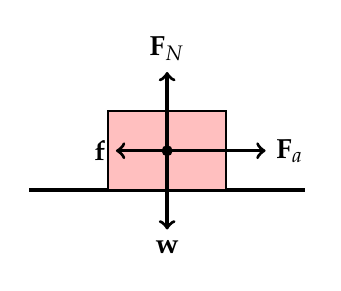
\begin{tikzpicture}
        \draw [very thick] (-1,0)--(2.5,0);
        \draw [fill=pink,thick] (0,0) rectangle (1.5,1);
        \fill (.75,.5) circle(2pt);
        \draw[->,very thick](.75,.5)--(.75,-.5) node[pos=1,below]{$\mb{w}$};
        \draw[->,very thick](.75,.5)--(.75,1.5) node[pos=1,above]{$\mb{F}_N$};
        \draw[->,very thick](.75,.5)--(2.,.5) node[pos=1,right]{$\mb{F}_a$};
        \draw[->,very thick](.75,.5)--(.1,.5) node[pos=1,left]{$\mb{f}$};
      \end{tikzpicture}
    \end{center}

    \column{.6\textwidth}
    \begin{center}
      \begin{tikzpicture}[scale=.5]
        \draw[very thick,->](0,0)--(10,0) node[pos=1,right]{$F_a$};
        \draw[very thick,->](0,0)--(0,5) node[pos=1,left]{$f$};
      \end{tikzpicture}
    \end{center}
  \end{columns}
\end{frame}



\begin{frame}{Drag}
  \textbf{Drag} (or \textbf{fluid resistance}) is the force opposing the
  motion of an object moving in a fluid, with a magnitude of:

  \eq{-.2in}{
    D=\frac{1}{2}\rho V_\infty^2A_\mathrm{ref}C_d
  }  
  \begin{center}
    \begin{tabular}{l|c|c}
      \rowcolor{pink}
      \textbf{Quantity} & \textbf{Symbol} & \textbf{SI Unit} \\ \hline
      Magnitude of drag force & $D$  & \si{\newton}\\
      Density of the fluid & $\rho$ & \si{\kg/\m^3}\\
      Free-stream fluid velocity & $V_\infty$ & \si{\m/\s}\\
      Reference area   & $A_\mathrm{ref}$ & \si{m^2}\\
      Drag coefficient & $C_d$ & (no unit)
    \end{tabular}
  \end{center}
  Drag coefficient depends on the shape and surface smoothness
  of the object. For blunt objects $A_\mathrm{ref}$ is the frontal area; for
  streamlined objects $A_\mathrm{ref}$ is the planform (top-view) area.
\end{frame}



\begin{frame}{Drag}
  In AP Physics you are not explicitly asked to know the drag equation.
  However, you should know that drag (air resistance) depends on the motion of
  the object and is not a constant.
\end{frame}


\begin{frame}{Terminal Velocity}
  When we take drag force into account, we understand that the drag force
  increases as an object speeds up, and therefore a free-falling object does
  \emph{not} accelerate infinitely. Instead it reaches a
  \textbf{terminal velocity}.

  \begin{columns}
    \column{.33\textwidth}
    
    {\footnotesize There is no air resistance just as the object \emph{begins}
      to fall. Acceleration is due to gravity alone.\par}

    \vspace{-.15in}
    \begin{center}
      \begin{tikzpicture}[scale=.9]
        \draw[very thick,->](0,0)--(0,-1.5) node[pos=1,below]{$\mb{w}$};
        \draw[very thick,->,white](0,0)--(0,1.5) node[pos=1,above]{$\mb{D}$};
        \fill(0,0) circle(0.07);
      \end{tikzpicture}
    \end{center}
    
    \column{.33\textwidth}

    {\footnotesize Drag increases as $v$ increases. Magnitude of acceleration
      decreases, but the object continues to gather speed\par}

    \vspace{-.15in}
    \begin{center}
      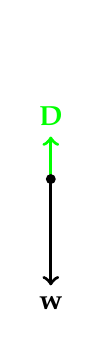
\begin{tikzpicture}[scale=.9]
        \draw[very thick,->](0,0)--(0,-1.5) node[pos=1,below]{$\mb{w}$};
        \draw[very thick,->,white](0,0)--(0,1.5) node[pos=1,above]{$\mb{F}_d$};
        \draw[very thick,->,green](0,0)--(0,.6) node[pos=1,above]{$\mb{D}$};
        \fill(0,0) circle(0.07);
      \end{tikzpicture}
    \end{center}
    
    \column{.33\textwidth}
    
    {\footnotesize Terminal velocity is reached when the drag force equals the
      object's weight. Not net force; no acceleration.\par}

    \vspace{-.15in}
    \begin{center}
      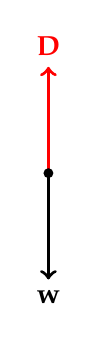
\begin{tikzpicture}[scale=.9]
        \draw[very thick,->](0,0)--(0,-1.5) node[pos=1,below]{$\mb{w}$};
        \draw[very thick,->,red](0,0)--(0,1.5) node[pos=1,above]{$\mb{D}$};
        \fill(0,0) circle(0.07);
      \end{tikzpicture}
    \end{center}
        
  \end{columns}
\end{frame}




%\begin{frame}{Example Problem}
%  \textbf{Example 8:} To move a \SI{45}{kg} wooden crate across a wooden floor
%  ($\mu=0.20$), you tie a rope onto the crate and pull on the rope. While you
%  are pulling the rope with a force of \SI{115}{N}, it makes an angle of
%  \ang{15}
%  with the horizontal. How much time elapses between the time at which the
%  crate just starts to move and the time at which you are pulling it with a
%  velocity of \SI{1.4}{m/s}?
%  \begin{center}
%    \pic{.5}{graphics/pull-box.png}
%  \end{center}
%\end{frame}
%
%\begin{frame}{Example Problem}
%  \textbf{Example 9:} You are holding an \SI{85}{kg} trunk at the top of a ramp
%  that slopes from a moving van to the ground, making an angle of \ang{35} with
%  the ground. You lose your grip and the trunk begins to slide.
%  \begin{itemize}
%  \item If the coefficient of friction between the trunk and the ramp is
%    $0.42$, what is the acceleration of the trunk?
%  \item If the trunk slides \SI{1.3}{m} before reaching the bottom of the ramp,
%    for what time interval did it slide?
%  \end{itemize}
%\end{frame}
%
%\begin{frame}{Example: Vertical Motion}
%  \textbf{Example 10:} A \SI{55}{kg} person is standing on a scale in an
%  elevator. If
%  the scale is calibrated in \emph{newtons}, what is the reading on the scale
%  when the elevator is not moving? If the elevator begins to accelerate upward
%  at \SI{.75}{m/s^2}, what will be the reading on the scale?
%\end{frame}


\begin{frame}{Tension in a Cable}
  \textbf{Tension} is the force exerted on and by a cable, rope,
  or string.

  \begin{itemize}
  \item You can't push on a rope
  \item Assume the cable/rope/string to be mass less
  \item Force can change direction when used with pulleys
  \end{itemize}
\end{frame}



\begin{frame}{Spring Force}
  The spring force $F_e$ is the force a compressed or stretched spring
  exerts onto objects connected to it. It obeys Hooke's Law:
  
  \eq{-.2in}{
    \mb{F}_e=-k\mb{x}
  }
  where $\mb{x}$ is the relative displacement of the ends of the spring.
  \begin{center}
    \pic{.35}{graphics/spring-example1.png}
  \end{center}
\end{frame}


\begin{frame}{Spring Force}
  \begin{center}
    \pic{.28}{graphics/spring-example1.png}
  \end{center}
  \begin{itemize}
  \item\vspace{-.15in}As the object falls onto the spring, the spring begins to
    compress
  \item As the spring compresses, the spring force (pointing up!) increases
    linearly (Hooke's law)
  \item At some point, the spring force balances the weight of the block
    \begin{itemize}
    \item At this point, the \emph{acceleration} is zero
    \item But the velocity continues to be downward
    \end{itemize}
  \item The spring continues to compress until velocity is zero
  \end{itemize}
\end{frame}



\begin{frame}{Spring Force}
  \begin{center}
    \pic{.28}{graphics/spring-example1.png}
  \end{center}
  \begin{itemize}
  \item\vspace{-.15in}Solving this problem using dynamics is difficult, because:
    \begin{itemize}
    \item Spring force scales linearly with \emph{displacement}, but
    \item Net force scales linearly with \emph{acceleration}
    \end{itemize}
  \item The block continues to \emph{increase} velocity even after
    it starts to compress the spring.
  \item Acceleration is zero only after the spring has compressed some amount
  \end{itemize}
\end{frame}



\begin{frame}{Buoyancy}{Everything Floats a Little}
  When an object is submerged inside a fluid (e.g.\ water, air, etc), the fluid
  exerts a pressure at the surface of the object. We can find the total buoyant 
  force $\mb{B}$ the fluid exerts on the object.
  \begin{center}
    \pic{.25}{graphics/rock_fbvectors.png}
  \end{center}
\end{frame}



\begin{frame}{Buoyancy}
  \framesubtitle{Everything Floats a Little}
  The buoyant force is given by:
  
  \eq{-.1in}{
    \boxed{\mb{B}=\rho_\mathrm{fluid}gV\bm{\hat{k}}}
  }
  \begin{center}
    \begin{tabular}{l|c|c}
      \rowcolor{pink}
      \textbf{Quantity} & \textbf{Symbol} & \textbf{SI Unit} \\ \hline
      Buoyant force & $\mb{B}$  & \si{\newton} \\
      Density of the fluid & $\rho_\mathrm{fluid}$ & \si{\kg/\m^3}\\
      Volume of the object & $V$ & \si{\metre^3}
    \end{tabular}
  \end{center}
  We will discuss this later in the course, when we deal with fluid mechanics.
\end{frame}



\section{Free-Body Diagrams}


\begin{frame}{Free Body Diagrams}
  \begin{itemize}
  \item Acceleration (if there is going to be any at all) depends
    on net force $\mb{F}_\mathrm{net}$
  \item Without a vector sum of all the forces, we cannot determine the
    magnitude, direction of the acceleration, or how acceleration will evolve
    in time
  \item We use \textbf{free body diagrams} (FBD) to represent all the forces.
    \begin{itemize}
    \item Very important in solving any dynamics problems
    \item Don't try to save this step, even if the problem does not ask for it
    \item Always draw FBD for solving classical mechanics problem
    \end{itemize}
  \end{itemize}
\end{frame}



\begin{frame}{Free Body Diagrams}
  In Grade 11/12 Physics, for rectilinear motion (no \emph{rotational motion}),
  FBDs are usually drawn by assuming that all forces acting at the CM,
  represented by the ``big dot''. For example:
  \begin{center}
    \vspace{-.15in}
    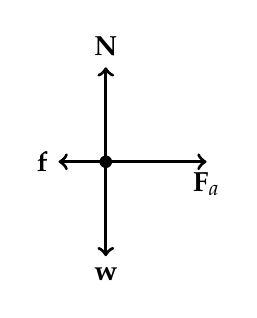
\begin{tikzpicture}[scale=.8]
      \fill (1.5,1) circle(.1);
      \draw [->,very thick] (1.5,1)--(1.5,-.5) node[pos=1,below]{$\mb{w}$};
      \draw [->,very thick] (1.5,1)--(1.5,2.5) node[pos=1,above]{$\mb{N}$};
      \draw [->,very thick] (1.5,1)--(3.1,1) node[pos=1,below]{$\mb{F}_a$};
      \draw [->,very thick] (1.5,1)--(.75,1) node[pos=1,left]{$\mb{f}$};
    \end{tikzpicture}
  \end{center}
  \vspace{-.1in}We can still use this method for rectilinear motion. However,
  this is not entirely correct. We notice that:
  \begin{itemize}
  \item Gravitational force $\mb{w}$ acts at the CM, but
  \item Normal force $\mb{N}$, friction $\mb{f}$ and applied force $\mb{F}_a$
    act at the point of contact
  \end{itemize}
\end{frame}



\begin{frame}{Free Body Diagrams}
  Instead, forces should be drawn at the point where they are applied. For
  example, a sphere rolling down a ramp should have weight $\mb{w}$, normal
  force $\mb{N}$ and static friction $\mb{f}_s$ acting on it:
  \begin{center}
    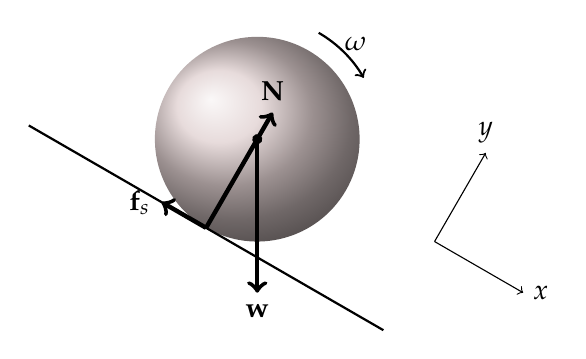
\begin{tikzpicture}[scale=1.3]
      \begin{scope}[rotate=-30]
	    \tikzstyle{balloon}=[ball color=gray!50!pink!50];
	    \shade[balloon](0,0) circle(1);
	    \draw[thick](-2,-1)--(2,-1);
	    %\draw[->,rotate=30](0,0)--(-1,0) node[pos=1,left]{$R$};
	    \draw[thick,->](0,1.2) arc(90:60:1.2) node[pos=.3,right]{$\omega$};
	    \fill(0,0) circle(.05); % node[right]{\small CM};
	    \draw[->,ultra thick,rotate=30](0,0)--(0,-1.5)
	    node[pos=1,below]{$\mb{w}$};
	    \draw[->,ultra thick](.0,-1)--(.0,.3)  node[pos=1,above]{$\mb{N}$};
	    \draw[->,ultra thick](.0,-1)--(-.5,-1) node[pos=1,left]{$\mb{f}_s$};
	    \draw[->](2,0)--(3,0) node[pos=1,right]{$x$};
       \draw[->](2,0)--(2,1) node[pos=1,above]{$y$};
	  \end{scope}
	\end{tikzpicture}
  \end{center}
  Once the FBD is drawn, decide on the axes to help you solve the motion. One of
  the axes should line up with the direction of motion. This guarantees that the 
  \emph{other} axis will not have any net force
\end{frame}



\begin{frame}{Example Problem}
  A more difficult static problem may involve two surfaces with two different
  friction coefficients. For example, a ladder leaning on a wall. This problem
  cannot be solved without first understanding rotational motion, but we can
  still draw a FBD.
  \vspace{.2in}
  \begin{columns}
    \column{.75\textwidth}
    \textbf{Example:} A uniform ladder is \SI{5.}{\metre} long and weighs
    \SI{400}{\newton}. The ladder rests against a slippery vertical wall, as
    shown in Figure. The inclination angle between the ladder and the rough
    floor is \ang{53}. Find the reaction forces from the floor and
    from the wall on the ladder and the coefficient of static friction $\mu_s$
    at the interface of the ladder with the floor that prevents the ladder from
    slipping.

    \column{.25\textwidth}
    \pic{1}{graphics/ladder.png}
  \end{columns}
\end{frame}



\section{Multi-Body Problems}

\begin{frame}{Applying Third Law of Motion on Connected Bodies}
  \begin{center}
    \pic{.7}{graphics/worldslongestroadtrainwithpowertrailer8.jpg}
  \end{center}
  \begin{itemize}
  \item The objects are connected by a cable or a solid linkage with negligible
    mass
  \item All objects (usually) have the same acceleration
  \item Require multiple free-body diagrams
  \end{itemize}
\end{frame}



\begin{frame}{Solving Connected-Bodies Problems}
  To solve a connected-bodies problem, you can follow these procedures:
  \begin{enumerate}
  \item Draw a FBD on each of the objects
  \item Sum all the forces on all the objects along the direction of motion
    \begin{itemize}
    \item Direction of motion is usually very obvious
    \item All internal forces should cancel and do not figure into the
      acceleration of the system
    \end{itemize}
  \item Compute the acceleration of the entire system using Newton's second law
    \begin{itemize}
    \item Remember that (usually) every object has the same acceleration!
    \end{itemize}
  \item Go back to the FBD of each of the objects and compute the unknown
    forces (usually tension)
  \end{enumerate}
\end{frame}



\begin{frame}{Connected Bodies: Example}
  \textbf{Example:} A tractor-trailer pulling two trailers starts from rest
  and accelerates with an acceleration $a$ on a straight, level road.
  The mass of the truck itself (T) is  %$m_T$, while the masses of the are
  %equal
  \SI{5450}{kg}, the
  mass of the first trailer (A) is \SI{31500}{kg}, and the mass of the second
  trailer (B) is \SI{19600}{kg}.
  \begin{enumerate}
  \item What magnitude of force must the truck generate in order to accelerate
    the entire vehicle?
  \item What magnitude of force must each of the trailer hitches withstand
    while the vehicle is accelerating?
  \end{enumerate}
  Assume that frictional forces are negligible in comparison with the forces
  needed to accelerate the large masses.
\end{frame}


\begin{frame}{Connected Bodies}
  Other type of connected bodies problem may be like this

  \vspace{.2in}
  \begin{columns}
    \column{.5\textwidth}
    Multiple objects pressed against one another:
    \begin{center}
      \begin{tikzpicture}[scale=.8]
        \draw(-1,0)--(5.5,0);
        \draw(0,0) rectangle(1,1);
        \draw(1,0) rectangle(3,1.5);
        \draw(3,0) rectangle(4.5,2);
        \draw[very thick,->](-1.5,.5)--(0,.5) node[pos=0,left]{$\mb{F}_a$};
      \end{tikzpicture}
    \end{center}
    
    \column{.5\textwidth}
    Multiple objects stacked on top of one another:
    \begin{center}
      \begin{tikzpicture}[scale=.8]
        \draw(-1,0)--(5.5,0);
        \draw(0,0) rectangle(4.5,1);
        \draw(1,1) rectangle(3.5,1.5);
        \draw(2,1.5) rectangle(2.5,2);
        \draw[very thick,->](4.5,.5)--(6,.5) node[pos=1,right]{$\mb{F}_a$};
      \end{tikzpicture}
    \end{center}
  \end{columns}
\end{frame}


\section{Pulley Problems}

\begin{frame}{Example Problem: Atwood Machine}
  An \textbf{Atwood machine} is made of two objects connected by a rope that
  runs over a pulley. The pulley allows the direction of force and direction
  of motion to change between two objects.
  \begin{columns}
    \column{.35\textwidth}
    \begin{center}
      \pic{1}{graphics/pulley_prob_2.png}
    \end{center}
    \column{.65\textwidth}
    \textbf{Example:} The object on the left has a mass of $M$ and the object
    on the right has a mass of $m$.
    \begin{itemize}
    \item What is the acceleration of the masses?
    \item What is the tension in the rope?
    \end{itemize}
  \end{columns}
\end{frame}


\begin{frame}{A Slightly More Difficult Problem}
  \begin{columns}
    \column{.35\textwidth}
    \pic{1}{graphics/pulley_prob_5.png}
    
    \column{.65\textwidth}
    Two blocks of mass $m$ and $M$ are connected via pulley with a
    configuration as shown on the left. The coefficient of static friction is
    $\mu_s$, between blocks and surface. What is the maximum mass $m$ so that
    no sliding occurs?
  \end{columns}
\end{frame}



%\begin{frame}{A Difficult Problem!}
%  \begin{columns}
%    \column{.6\textwidth}
%    \textbf{Example:} Two blocks of mass $m$ and $M$ are connected via pulley
%    with a configuration as shown on the right. The coefficient of static
%    friction between the left block and the surface is $\mu_{s,1}$, and the
%    coefficient of static friction between the right block and the surface is
%    $\mu_{s,2}$. Formulate a mathematical inequality for the condition that no
%    sliding occurs. There may be more than one inequality. 
%    
%    \column{.4\textwidth}
%    \pic{1}{graphics/pulley_prob_6.png}
%  \end{columns}
%\end{frame}



%\begin{frame}{Multiple Pulleys}
%  When there are multiple pulleys involved, we have to remember that tension
%  force is distributed evenly along the cable.
%
%  \vspace{.2in}
%  \begin{columns}
%    \column{.6\textwidth}
%    \textbf{Example:} A block of mass $m$ is pulled, via two pulleys as shown,
%    at constant velocity along a surface inclined at angle $\theta$. The
%    coefficient of kinetic friction is $\mu_k$, between block and surface.
%    Determine the pulling force $F$. Ignore the mass of the pulleys. 
%    
%    \column{.4\textwidth}
%    \pic{1}{graphics/pulley_prob_7.png}
%  \end{columns}  
%\end{frame}
%
%
%\begin{frame}{One More!}
%  \begin{columns}
%    \column{.75\textwidth}
%    \textbf{Example:} A block of mass $M$ is lifted at constant velocity, via
%    an arrangement of pulleys as shown. Determine the pulling force $F$. Ignore
%    the mass of the pulleys. 
%
%    \uncover<2>{
%      \vspace{.2in}\textbf{Example:} The pulling force is replaced by a $10M$
%      mass, and was let go. What are the accelerations of the $M$ and the
%      $10M$ mass?
%    }
%    
%    \column{.25\textwidth}
%    \pic{1}{graphics/pulley_prob_9.png}
%  \end{columns}
%\end{frame}


%\begin{frame}{A More Typical Problem}
%  \textbf{Example 14:}
%  More typically, an Atwood machine problem is one where two objects are
%  sliding on a surface. These surfaces may have (or may not) have friction.
%  In this example, two blocks are connected by a mass-less string over a
%  friction-less pulley as shown in the diagram.
%  \begin{columns}
%    \column{.45\textwidth}
%    \begin{tikzpicture}[scale=.8]
%      \draw[thick](0,0)--(-4,0) node[midway,below]{\tiny $\mu_k=0.14$};
%      \draw(-1.75,0) rectangle(-3,.75) node[midway]{\tiny\SI{0.80}{\kg}};
%      \draw(-1.75,.44)--(.1,.44);
%      \begin{scope}[rotate=-30]
%        \draw[thick](0,0)--(5,0) node[midway,left]{\tiny $\mu_k=0.14$};
%        \draw(3,0) rectangle(4.25,.75) node[midway]{\tiny\SI{2.}{\kg}};
%        \draw(3,.44)--(-.05,.44);
%      \end{scope}
%      \begin{scope}[rotate=-15]
%        \draw (0,0)--(0,.3);
%        \draw (0,.3) circle(.15);
%      \end{scope}
%      \draw[gray!50](0,0)--(0,-2);
%      \draw[->](0,-.5)arc(270:330:.5)node[midway,right]{\tiny\ang{60}};
%    \end{tikzpicture}
%    \column{.55\textwidth}
%
%    \begin{enumerate}[(a)]
%    \item Determine the acceleration of the blocks.
%    \item Calculate the tension in the string.
%    \item If the string broke, for what minimum value of the coefficient of
%      static friction would the \SI{2.}{kg} block not begin to slide?
%    \end{enumerate}
%  \end{columns}
%\end{frame}
\end{document}
